\documentclass[11pt,a4paper]{article}
\usepackage[latin1]{inputenc}
\usepackage{amsmath}
\usepackage{amsfonts}
\usepackage{amssymb}
\usepackage{graphicx}
\usepackage{geometry}
\usepackage{xcolor}

%\usepackage{showframe} %This line can be used to clearly show the new margins

\newgeometry{vmargin={30mm}, hmargin={25mm,25mm}} 
\setlength{\topskip}{0mm}

\begin{document}
\title{\textbf{Response to Reviewer 2}}
\date{}
\maketitle	

The authors would like to thank the reviewer for his/her careful review and constructive comments, which we believe will help improve the content of the manuscript.  Below, under each bullet point, we provide a point by point response to each comment/question. The author responses are given in blue, and textual changes are italicised.  

\section*{General Comments}
\begin{itemize}

\item 			
			As I understand it, this study uses only simulated measurements (either with or without hydrometeors included), even for MWHS-2 for which actual measurements are available. This should be made clearer, especially given line 66, which states that no``background'' data is required for the method. I'd also like to see a bit more discussion 	about whether the results you present should be expected to hold for real data. An assumption that you are making is that your forward model can represent real clouds with enough fidelity that a model trained on simulated data will still work on real-world data. Can you point to any evidence to back up this assumption? Have you tried comparing the histograms of model-simulated Tbs with real-world MWHS-2 Tbs?\\


\textcolor{blue}{Reply: We agree with the reviewer, the line 66, can be confusing. We have re-written the sentence to:\\
Pg 3, line 68:	``\textit{This is done for each channel separately and by only using the measurements, although the scheme is demonstrated in the study by using simulated observations.}''\\\\		
Regarding the discussion about simulations holding well for the real-data, we agree with the reviewer that our assumption is a strong one and requires some evidence. For MWHS-2, we have added a new figure (Pg 6, Fig. 1, also shown below) comparing the histograms of background and bias corrected observations for one of the lower peaking channels of 183 GHz channel.  The main deviations in the distributions arise from the hydrometeor scattering. With limited scope of particle size and shape variation in current NWP microphysical schemes, the true cloud variability cannot be  described accurately, and a bias correction is necessary to be closer to the reality. Also, ECMWF has real time monitoring of many satellite sensors including FY-3D MWHS-2, thus it is possible to assess how well the system (and RTTOV-SCATT) is performing.
\newline
For ICI and SMS, though a qualitative assessment of the simulations is not possible, we expect underestimation of the cloud variability owing to only single PSD and habit assumption. However, it is important to consider that QRNN can easily adapt to changes in brightness temperatures introduced by PSD and habit variation.\\
We have added this discussion in the revised manuscript in Sect 2.2. }\\
\begin{figure}
	\centering
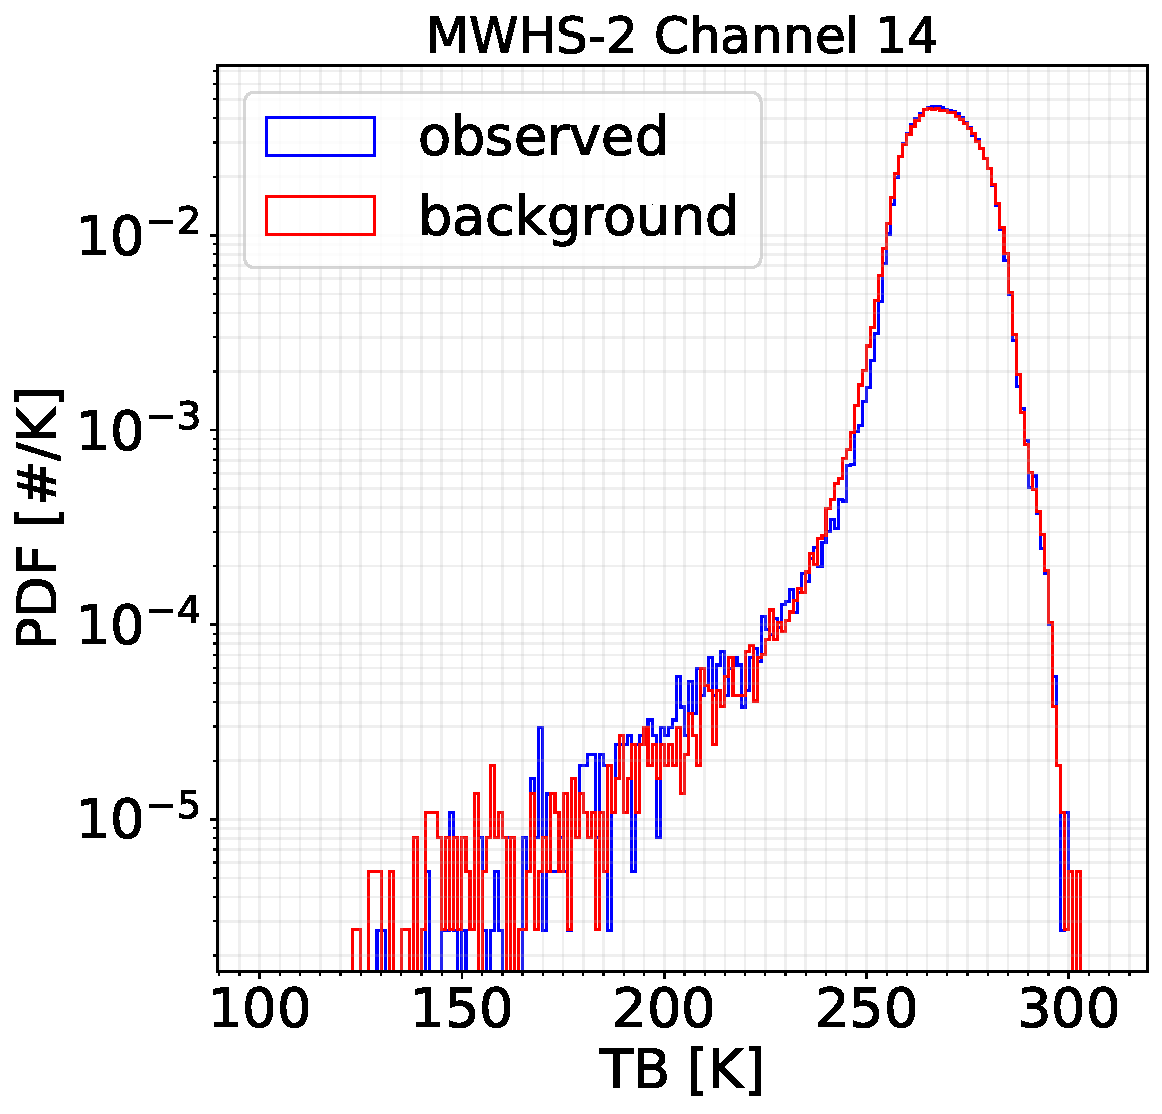
\includegraphics[width = 80mm]{fig00.pdf}
\caption{Probability distribution functions (PDFs) of simulated and observed brightness temperatures for MWHS-2 channel 14. The data covers latitude range $60^{\circ}$\,S to $60^{\circ}$\,N, and satellite zenith angle less than $7.5^{\circ}$.}
\end{figure}
		
\item  	
			What is the computational cost of the QRNN method compared to simpler cloud-
			clearing filters? Could it feasibly be implemented into existing NWP models given
			current computational constraints?\\

\textcolor{blue}{Reply: Yes, it would be feasible to implement the scheme into existing NWP models. In this study, QRNN was not optimized to get the maximum computational performance. For each MWHS-2 channel, it took around 30 minutes to train the net on a  x86\_64, 8 CPU machine. For ICI and SMS, with smaller training dataset, the time was lower. However, with the modern computing architectures and parallel processing, a much faster computation can be expected. }\\

\item  
			Lines 135-143: Why the large difference in number of cases simulated for ICI (220\,000)
			vs. SMS (143\,000), if they are both coming from the same population of CloudSat
			profiles? For the training dataset, you use about 75\% of total cases for MWHS-2,
			about 80\% of cases for ICI, and about 84\% of cases for SMS. Why this difference in
			proportions?\\

\textcolor{blue}{Reply: Yes, both ICI and SMS simulations come from same population of Cloudsat. For SMS, we had access to a smaller database, which was used for a earlier study. Due to difference in sizes of the available observations, maximum possible observations were incorporated in the training data to allow cloud variability. Even with differences in the database sizes, the results show that the predicted quantiles are well calibrated for all three sensors. With a larger database, one could expect similar or even better performance.}\\

\item  
			Line 340: ``With a test dataset of 70 000 samples, we cannot represent the far wings of the distribution accurately.'' Couldn't one apply this same reasoning to Figures 2,3, or
			8, which have density values below $10^{-4}$ included?\\

\textcolor{blue}{Reply: Yes one could apply the same reasoning to the Figures 2, 3, or 8, but we prefer to show the complete distribution to emphasize that the cases with large errors occur infrequently.}\\


\item 
			Figure 13: I wonder if there might be an easier, more concise way to evaluate whether
			the uncertainty intervals are properly calibrated. Namely, could you simply calculate
			how often the true value falls within the $\pm2\sigma$ uncertainty range, for each of the uncertainty bins ($0 - 3$K, $3 - 8$K, $8 +$ K) that you've included on the plot? If this percentage is significantly less than 95\%, it would suggests that your uncertainties are too small, while if it were closer to 100\% it would suggest your uncertainties are too large. Even if you don't get rid of Fig. 13, I think this would be useful information to include in the paper.\\

\textcolor{blue}{Reply: As per suggestion of the reviewer, we have included the information highlighting how well calibrated the uncertainties are. We provide the occurence percentage of true value for each uncertainty bin and add this information in Fig. 13 (also shown above). For each bin considered, the true value falls in the range almost 94\% of the time, indicating that the uncertainties are well calibrated. Only for channel I3V and the outermost bin, occcurence percentage is 88\%. \\	
These results are in line with Fig.7 and Fig.11, which also indicate that the uncertainty intervals are well calibrated.} \\
\begin{figure}
	\centering
	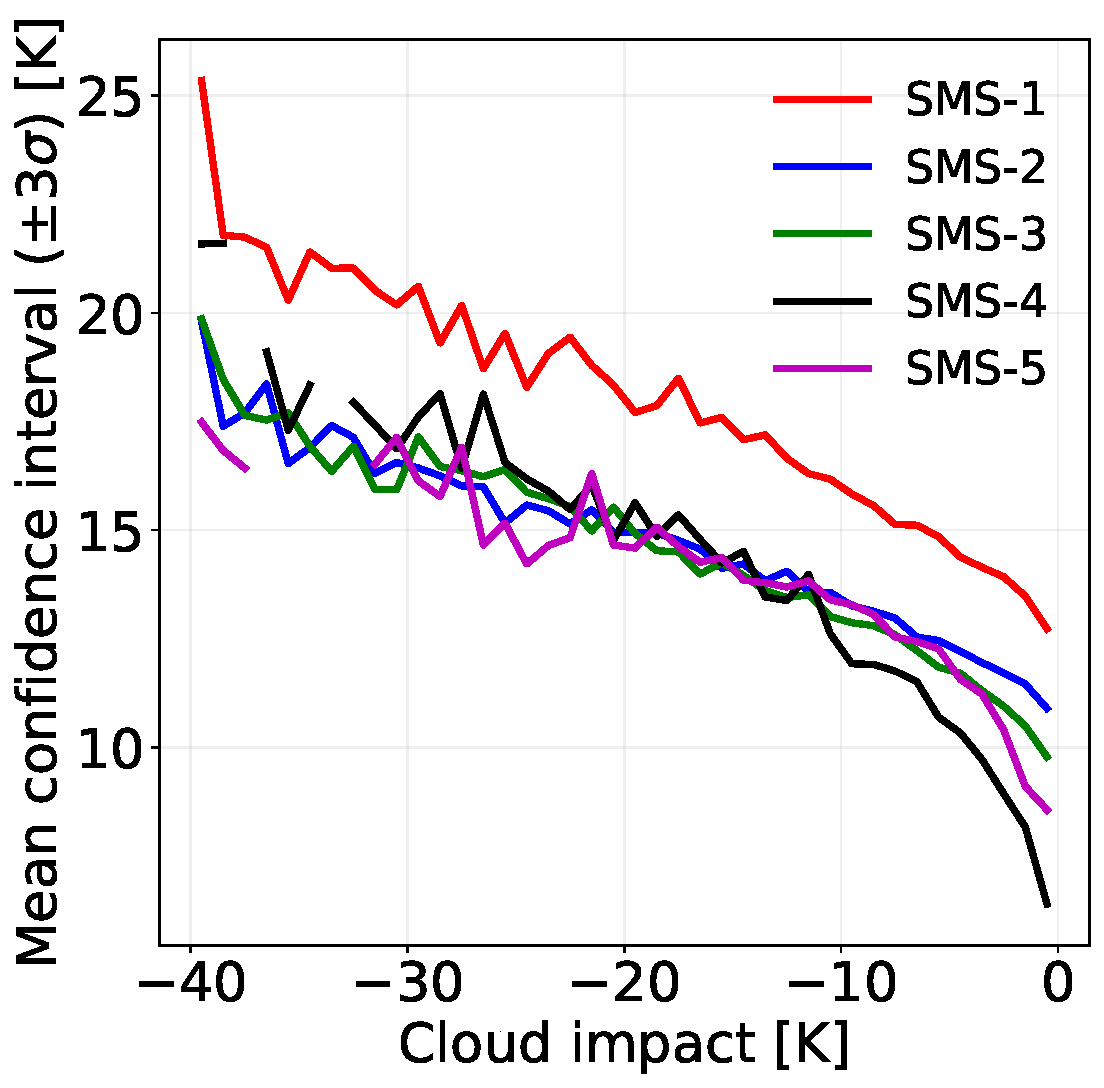
\includegraphics[width = 190mm]{fig13.pdf}
	\caption{Distribution of errors binned according to their uncertainty. The occurrence of true value in each uncertainty interval bin is given in the parentheses. Results are from QRNN-single for channels I1V, I2V and I3V.}
\end{figure}
\item  
			Lines 498-499: ``. . . other underlying uncertainties not considered here.'' Whether here or elsewhere in the paper, I think you should talk a bit more about what these other uncertainties are (radiative transfer model errors should certainly be discussed), and what effects they might have on your results.\\

\textcolor{blue}{Reply: Among the errors which affect the radiative transfer calculations are underestimation of cloud variability due to limited particle size distribution (PSD) and habit variation. Other factors include neglected antenna pattern and the limitations associated with input data, both Cloudsat and ERAInterim. For example, the simulations could have tendency to be biased towards the Cloudsat geographical sampling. All these issues can contribute to mapping errors between 183\,GHz  and higher frequency channels. However, it is possible improve the cloud representation by incorporating PSD and habit variation, and QRNN based cloud correction can easily adapt to changes in brightness temperatures introduced by the local variability.  This is not the case with all-sky data assimilation systems, which assume only single PSD and habit combination, and shall continue to do so in coming years.\\
We have edited Sect 2.2 and Conclusions to describe these different errors and their implications.  }	

\end{itemize}
	
\section*{Typos}
\begin{itemize}


\item Line 26: The phrase ``weather satellites are since some time equipped'' is confusing to
me. I suggest ``weather satellites have for some time been equipped. . .''

\textcolor{blue}{Reply: The sentence is re-written as per suggestion.}

\item Line 51: I believe you are missing the word ``on'' between ``predicated'' and ``Gaussian.''

\textcolor{blue}{Reply: The typo is corrected.}

\item Line 154: Should 85\% be changed to 84\%? That would be +2 sigma for a normal
distribution.

\textcolor{blue}{Reply: Yes, the predicted percentile should be 84\% instead of 85\%. The typo is corrected.} 


\item Line 455:``. . . provide coverage to the humidity channels in, lower and mid troposphere''
This is confusing - get rid of the comma and add the word ``the'' instead?

\textcolor{blue}{Reply: The comma is removed and the word ``the'' is added.}


\item Line 494:	``QRNN predictions are weighted mean. . .'' I think this should say, ``QRNN
predictions are the weighted mean. . .''

\textcolor{blue}{Reply: The word ``the'' is added.}



\item Line 508: Missing ``the'' before ``same''


\textcolor{blue}{Reply: The word ``the'' is added.}

\end{itemize}
	
\end{document}